\section{Roads and Urban Networks} \label{sec:Roads}
We are able to apply the PageRank algorithm to road networks in order to predict traffic flow and also human movement. Jiang et al. found that Weighted PageRank, as discussed in Section \ref{sec:weighted} of this report, is the best metric with regards to correlating or predicting traffic flow \cite{1742-5468-2008-07-P07008}. A city can be topologically represented by a connectivity graph as shown in Figure \ref{fig:city rep}, and as over 60\% of human movement can be predicted or explained using a connectivity graph \cite{doi:10.1080/13658810802022822}.

\begin{figure}[h!]
\centering
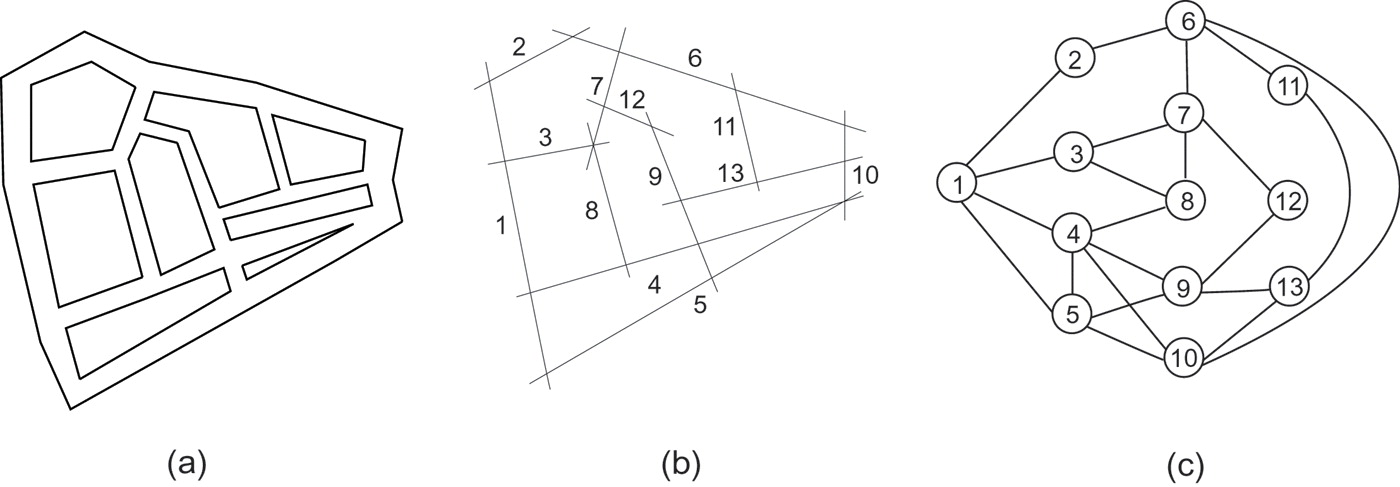
\includegraphics[width=\linewidth]{map_view.jpeg}
\caption{(a) A fictive urban system, (b) its axial map and (c) connectivity graph, taken from \cite{doi:10.1080/13658810802022822}}
\label{fig:city rep}
\end{figure}

This application is slightly different to the usual PR algorithm, as the graph formed from a urban space is a connected graph, and so there are no dangling nodes involved, in terms of a random walker, they will never get stuck, we assume that they never get tired and that they always move to one of its successors with non-uniform probability, as well-connected streets are preferable. Due to this non-uniform probability, we need to use the WPR algorithm as discussed in Section \ref{sec:weighted} as opposed to the standard algorithm.
